\section{Measurement and Density/Relative Density}	

%Concept of Measurement

\subsection{Construction of a Metre Rule}
\label{sub:metrerule}

\begin{description*}
\item[Subtopic:]{Concept of Measurement}
\item[Materials:]{Wooden board, pen\slash pencil, a handsaw, ruler or tape measure}
%\item[Setup:]{}
\item[Procedure:]{Use the handsaw to cut a piece of wood 100 cm $\times$ 3.5 cm $\times$ 0.5 cm. Use a ruler or tape measure to mark a scale in cm on the wood.}
%\item[Hazards:]{}
%\item[Questions:]{}
%\item[Theory:]{}
%\item[Applications:]{}
\item[Notes:]{Instead of a wooden block, string can be used by making knots at different intervals.}
\end{description*}

%\subsection{Construction of a Metre Rule}
%\label{sub:metrerule}
%
%\subsubsection*{Learning Objective}
%\begin{itemize}
%\item{To construct and use a metre rule.} 
%\end{itemize}
%
%\subsubsection*{Background Information}
%Length is an interval between two points. It is usually measured in metric units like the metre (m), millimetre (mm), centimetre (cm), kilometre (km).
%
%\subsubsection*{Materials}
%Wooden board, pen/pencil, a handsaw, ruler or tape measure
%
%\subsubsection*{Preparation Procedure}
%\begin{enumerate}
%\item{Use the saw to cut a piece of wood 100 cm x 3.5 cm x 0.5 cm.} 
%\item{Use a ruler to mark a scale in cm on the wood.} 
%\end{enumerate}
%
%\subsubsection*{Activity Procedure}
%Use the new metre ruler to measure length of different objects.
%
%\subsubsection*{Discussion Question}
%What other objects can be arranged in order to measure distance?
%
%\subsubsection*{Notes}
%Instead of a wooden block, string can be used by making knots at a definite intervals.


\subsection{Construction of a Measuring Cylinder}
\label{sub:meascyl}
\begin{description*}
\item[Subtopic:]{Concept of Measurement}
\item[Materials:]{Plastic bottles of different sizes, syringes (30 mL - 50 mL), marker pen, ruler, bucket of water}
%\item[Setup:]{}
\item[Procedure:]{Using the syringe, transfer a known volume of water from the bucket to the empty bottle. Use the marker pen to mark the level of water on the bottle. Repeat for a range of volumes, using a ruler to complete the scale.}
%\item[Hazards:]{}
%\item[Questions:]{}
%\item[Theory:]{}
%\item[Applications:]{}
%\item[Notes:]{}
\end{description*}

%\subsection{Construction of a Measuring Cylinder}
%\label{sub:meascyl}
%
%\subsubsection*{Learning Objective}
%\begin{itemize}
%\item{To construct and use a measuring cylinder.} 
%\end{itemize}
%
%\subsubsection*{Background Information}
%A measuring cylinders measures the volume of liquids in millilitres (mL).
%
%\subsubsection*{Materials}
%Plastic bottles of different sizes, syringes (30-50 mL), marker pen, ruler, bucket full of water
%
%\subsubsection*{Preparation Procedure}
%\begin{enumerate}
%\item{Using the syringe, take a known volume of water from the bucket.} 
%\item{Transfer the known volume of water in the syringe to the empty plastic bottle.} 
%\item{Using the marker pen, mark the level of water in the plastic bottle with the volume from the syringe.}
%\item{Repeat this step for a range of volumes, marking each volume on the side of the bottle.}
%\item{Use a ruler to complete the scale.} 
%\end{enumerate}
%
%\subsubsection*{Activity Procedure}
%Use the constructed measuring cylinder to measure volumes of different liquids.
%
%\subsubsection*{Clean Up Procedure}
%Remove waste and return materials to their proper places.
%
%\subsubsection*{Discussion Question}
%Explain how to use a measuring cylinder.
%
%\subsubsection*{Notes}
%A measuring cylinder cannot be used to measure the volume of a solid by itself, though if the solid is immersed in a liquid, the volume can be determined with a measuring cylinder. The volume of granular and porous materials can also be measured if they are immersed in a liquid in a measuring cylinder.

\subsection{Construction of Scale Pans}
\label{sub:scalepans}

\begin{center}
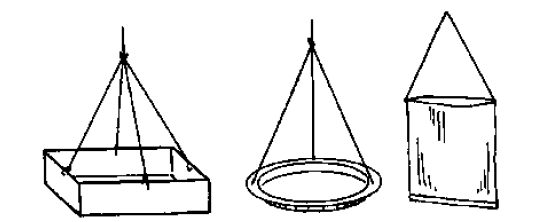
\includegraphics[width=10cm]{./img/source/scale-pans.png}
\end{center}

\begin{description*}
\item[Subtopic:]{Concept of Measurement}
\item[Materials:]{Match boxes, large plastic bottles, tin can lids, small plastic bags, knife, string}
%\item[Setup:]{}
\item[Procedure:]{Use a knife to poke 3~-~4 holes in the sides of one of the above materials. If using plastic bottles, cut them about 3~-~4~cm from the bottom. Cut equal lengths of string and tie them through the holes in the scale pan. Join the strings together at the upper end. }
%\item[Hazards:]{}
%\item[Questions:]{}
%\item[Theory:]{}
%\item[Applications:]{}
%\item[Notes:]{}
\end{description*}


\subsection{Construction of Beam Balance}
\label{sub:beambalance}

\begin{center}
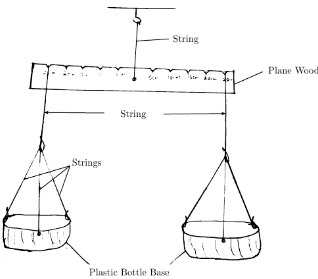
\includegraphics{./img/beam-balance.png}
\end{center}

\begin{description*}
\item[Subtopic:]{Concept of Measurement}
\item[Materials:]{Ruler or wooden bar 30 cm $\times$ 2 cm, razor/knife, string/wire, pen, 2 \nameref{sub:scalepans}, nails, heat source*}
%\item[Setup:]{}
\item[Procedure:]{Find the balancing point of the ruler/wood block and mark it with a pen. Use a heated nail to make a hole through this point. Make notches at 5 cm intervals on either side of the center hole using a razor/knife and suspend scale pans accordingly. Use a string/wire tied through the center hole to suspend the balance.}
%\item[Hazards:]{}
%\item[Questions:]{}
%\item[Theory:]{}
%\item[Applications:]{}
%\item[Notes:]{}
\end{description*}

%\subsection{Construction of Beam Balance}
%\label{sub:beambalance}
%
%\subsubsection*{Learning Objective}
%\begin{itemize}
%\item{To construct and use a beam balance.} 
%\end{itemize}
%
%\subsubsection*{Background Information}
%Mass is a fundamental quantity and is measured by using a beam balance. In physics mass is usually measured in grams (g) or kilograms (kg).
%
%\subsubsection*{Materials}
%Wooden bar 30 cm x 2 cm, string/wire, ruler, pencil/pen, 2 large plastic bottles, nails, heat source*
%
%\subsubsection*{Preparation Procedure}
%\begin{enumerate}
%\item{Cut a piece of wood block to 30 cm x 2 cm.} 
%\item{Find the balancing point and then mark the point using a pencil or pen.} 
%\item{Make a hole at the balance point using a hot nail.} 
%\item{Mark 5~cm spaces on each side of the hole using a ruler.} 
%\item{Cut 2 plastic bottles about 3~-~4~cm from the bottom.} 
%\item{Make 3 round holes in the bottom of a plastic bottle at equal intervals. These will be used as scale pans.} 
%\item{Tie pieces of thread/wire about 15 cm length into the holes of the bottom of a plastic bottle.} 
%\item{Join the upper ends of the thread/wires together.} 
%\item{Suspend the wooden block by using a piece of string/wire tied through the centre hole.} 
%\end{enumerate}
%
%\begin{figure}
%\begin{center}
%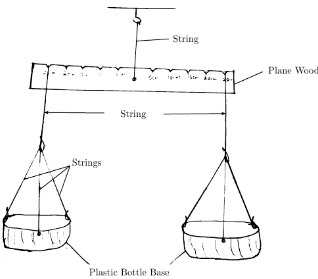
\includegraphics{./img/beam-balance.png}
%\caption{A beam balance}
%\label{fig:beam-balance}
%\end{center}
%\end{figure}
%
%\subsubsection*{Activity Procedure}
%Use the beam balance to measure the masses of different objects in the classroom.
%
%\subsubsection*{Clean Up Procedure}
%Return all materials to their proper places.
%
%\subsubsection*{Discussion Question}
%How can you improve the beam balance?
%
%\subsubsection*{Notes}
%There are different kinds of balances, such as a digital balance, double beam balance, single beam balance and triple beam balance. Each can be used to measure mass according to its sensitivity.



%\subsection{Making a Spring and a Spring Balance}
%
%\subsubsection*{Learning Objectives}
%\begin{itemize}
%\item{To make springs for various uses.}
%\item{To create and calibrate a spring balance.}
%\end{itemize}
%
%\subsubsection*{Background Information}
%Springs typically have a constant value which determines how much they can stretch or compress.  Because the value is constant, we can use it to accurately measure mass or weight, as it will always extend to the same length with the same force.
%
%\subsubsection*{Materials}
%Strong metal wire of swg 24 or 26 of various types like copper, nichrome or constantine; a rod of diameter 14 to 18 mm of any material, piece of wood, ruler, plane paper, known masses, glue.
%
%\subsubsection*{Preparation Procedure}
%Cut the metal wire into different lengths of at least 50 cm.
%
%\subsubsection*{Activity Procedure}
%\begin{enumerate}
%\item{Take a piece of wire and hold one end to the rod.}
%\item{Coil the wire tightly along the rod, keeping the coils close together.}
%\item{When the entire wire is coiled along the rod, remove the rod.}
%\item{Bend btoh ends of the wire into hooks.}
%\item{Repeat these steps for all of the wires of different types and lengths.}
%\item{Try stretching and compressing the springs to test the different strengths.}
%\item{Attach the end of one spring to the top of a piece of wood with a nail or screw.}
%\item{Glue or tape some white paper to the wood behind the spring.}
%\item{Use a pen to make a mark at the bottom of the spring.}
%\item{Hang a known mass on the spring so that it is stretched downward a short distance.}
%\item{Make a mark at the bottom of the spring in its new position.  Label this with the mass of the object hung from the spring.}
%\item{Repeat this process for other masses, marking each mass on the paper.}
%\item{Use a ruler to finish the scale by filling in masses above, below and between the marks you have made.}
%\end{enumerate}
%
%\begin{figure}
%\begin{center}
%\def\svgwidth{150pt}
%\input{./img/spring-balance.pdf_tex}
%\caption{A Spring Balance}
%\label{fig:spring-balance}
%\end{center}
%\end{figure}
%
%\subsubsection*{Results and Conclusions}
%When a load is placed on the spring, it increases the length of the spring.  When the load is removed, the spring returns to its original length.
%Different materials of the same swg have different spring constants (strengths), or force per extension length.
%
%\subsubsection*{Clean Up Procedure}
%Return all materials to their proper places.
%
%\subsubsection*{Discussion Questions}
%\begin{enumerate}
%\item{What are some uses of springs?}
%\item{What are the qualities of a good spring?}
%\item{What is the relationship between the wire's diameter and the strength of the spring?}
%\item{Which metal makes the strongest spring?  Which metal makes the weakest spring?}
%\end{enumerate}
%
%\subsubsection*{Notes}
%A good spring must obey Hooke's Law.  Springs can be used to make a spring balance or can be used in physics practicals to find the relationship between force and the resulting extension.


%Eureka Can

\subsection{Construction of Eureka Can}
\label{sub:eurekacan}

\begin{center}
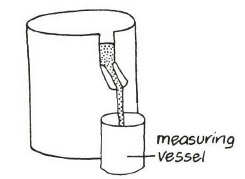
\includegraphics[width=6cm]{./img/vso/overflow-can.png}
\end{center}

\begin{description*}
\item[Subtopic:]{Determining the Volume of Irregular Objects}
\item[Materials:]{Plastic bottle, knife}
%\item[Setup:]{}
\item[Procedure:]{Cut a plastic bottle about 10~cm from the bottom. Cut 2 slits at the top of the bottle and bend the strip forward to form a spout.}
%\item[Hazards:]{}
%\item[Questions:]{}
%\item[Theory:]{}
\item[Applications:]{Measuring the volume of irregular objects, Archimedes' Principle}
\item[Notes:]{Alternatively, use a bottle or tin can and poke a hole near the top using a heated nail. Attach a straw/hollow pen tube/tube of aluminum foil, using super glue to ensure an air-tight seal.}
\end{description*}

%\subsubsection*{Learning Objectives}
%\begin{itemize}
%\item{To construct a eureka can and use it to measure volumes of irregular objects.} 
%\end{itemize}
%
%\subsubsection*{Materials}
%Plastic bottles of 500 mL or 1000 mL, straws* or a syringe needle cap, a knife/razor blade, heat source*, cellotape or super glue, nail, and a wire
%
%\subsubsection*{Preparation Procedure}
%\begin{enumerate}
%\item{Cut the plastic bottle in half and use the bottom part.} 
%\item{Heat a sharp pointed end of the nail.} 
%\item{Using the heated sharp point of the nail, make a small hole about 5 cm from the top of the cut plastic bottle.} 
%\item{Cut a piece of straw about 5 cm long or use the syringe needle cap.} 
%\item{Insert the piece of straw into the hole. Make sure the piece of straw is tightly fixed with cellotape or super glue.} 
%\end{enumerate}
%
%\subsubsection*{Activity Procedure}
%Use the constructed eureka can to overflow different liquids and to measure the volume of liquid displaced when an object floats in it.
%
%\subsubsection*{Clean Up Procedure}
%Collect all the used materials, cleaning and storing items that will be used later.
%
%\subsubsection*{Discussion Questions}
%\begin{enumerate}
%\item{What is the relationship between the weight of a floating object and the weight of water it displaces?}
%\item{What is the reason for using a Eureka Can instead of a normal bottle?}
%\end{enumerate}
%
%\subsubsection*{Notes}
%A Eureka Can is typically used to move a certain volume from the can into another container.  When an object floats in a liquid, it displaces its own weight in water.  If the level of water in the Eureka can is at the level of the spout, the water displaced will flow through the spout into another container.  This water can then be measured on a beam balance to find the weight of the object.


%Weight vs. Mass


%Density, Relative Density
	%See Density in Chem for more

\subsection{Applications of Material Densities}

\subsubsection*{Learning Objectives}
\begin{itemize}
\item{To observe the difference between densities of different liquids and solids.} 
\item{To design a density tower using a variety of liquids with different densities.} 
\end{itemize}

\subsubsection*{Background Information}
Materials can usually be distinguished from each other by their densities.  Normally, less dense materials float on denser liquids.  When liquids are placed in a container, the heavier (denser) liquids sink while the lighter (less dense) liquids float.  A density tower can be designed using liquids of different densities, even if they are soluble.

\subsubsection*{Materials}
Water, honey, glycerine, cooking oil, spirit, kerosene, beakers*, test tubes*, syringes, small pieces of wood, small pieces of rubber, small pieces of metal, and different food colour (optional).

\subsubsection*{Preparation Procedure}
\begin{enumerate}
\item{Find a test tube or syringe.}
\item{Place each liquid into a beaker so it can easily be obtained by students.} 
\end{enumerate}

\subsubsection*{Activity Procedure}
\begin{enumerate}
\item{Place a small amount of honey into the test tube.} 
\item{Slowly add glycerine to the test tube.} 
\item{Slowly pour water into the test tube.} 
\item{Slowly add methylated spirit to the test tube.} 
\item{Add cooking oil into the test tube.} 
\item{Slowly add kerosene to the test tube.} 
\item{Put a small piece of wood, rubber and iron into the test tube.}
\item{Observe the positions of the liquids and solids relative to each other.}

\end{enumerate}
\begin{figure}[h]
\begin{center}
\def\svgwidth{200pt}
\input{./img/density-tower.pdf_tex}
\caption{Density tower}
\label{fig:density-tower}
\end{center}
\end{figure}

\subsubsection*{Results and Conclusions}
The liquids with a higher density will sink, while the liquids with lower density will float. When the solid materials are dropped into the test tube, the solid material will rest in the liquid that has a relatively equal density.  

\subsubsection*{Clean Up Procedure}
Collect all materials and return them to their proper place.

\subsubsection*{Discussion Questions}
\begin{enumerate}
\item{Why should liquid be poured slowly into the test tube?}
\item{What happens when the wood, iron, and rubber are placed into test tubes?} 
\end{enumerate}

\subsubsection*{Notes}
Heavier density liquid should be poured into the test tube first, followed by relatively less dense liquids. Pouring the liquids should be done slowly to avoid mixing of liquid. Food colour can also be added to colorless liquid such as water, kerosene, and glycerine.  

\subsection{Relative Density of a Liquid}

\subsubsection*{Learning Objectives}
\begin{itemize}
\item{To determine the density and relative density of a liquid.} 
\end{itemize}

\subsubsection*{Background Information}
Bodies of different materials have different densities.  Density can be found by taking the ratio of a body's mass to its volume.  $$\mathrm{Density} = \frac{\mathrm{mass}}{\mathrm{volume}}$$

Relative density (R.D.) can be used to compare the density of a given material to that of water.  Water is the standard with a density of 1.0 g/mL, so all other densities are compared to water.
$$\mathrm{R.D.} = \frac{\mathrm{Density\; \; of \;substance}}{\mathrm{Density\; \;of \;water}}$$

\subsubsection*{Materials}
``Density bottle" (small empty can or bottle), rubber stopper/dry grass/maize cob*, plastic bag, water, honey, kerosene, cooking oil, straw/bamboo stick


\subsubsection*{Activity Procedure}
\begin{enumerate}
\item{Weigh the can with its stopper and plastic bag in air (variable \ce{M0}).} 
\item{Fill the small can with water and weigh it (variable \ce{M1}).} 
\item{Pour out the water from the can and dry it with a piece of clean cloth or tissue.} 
\item{Fill the can with another liquid, like honey, kerosene, or cooking oil, and weigh it again. (Variable \ce{M2})}
\item{Repeat steps 3 and 4 for other liquids}
\item Calculate the relative density of each liquid tested
\end{enumerate}

\subsubsection*{Results and Conclusions}
Mass of density bottle = \ce{M0}\\
Mass of density bottle with water = \ce{M1}\\
Mass of the density bottle with liquid A = \ce{M2}\\
$$\mathrm{Relative \;density \;of \;liquid \;}A = \frac{\mathrm{Mass \;of \;liquid \;}A}{\mathrm{Mass \;of \;water}} = \frac{M_2-M_0}{M_1-M_0}$$
We use this formula to find the relative density of any liquid.

\subsubsection*{Clean Up Procedure}
Collect all the used materials, cleaning and storing items that will be used later.

\subsubsection*{Discussion Questions}
\begin{enumerate}
\item{Determine the mass of the water.} 
\item{Calculate the volume of the density bottle and the relative density of honey.} 
\end{enumerate}

\subsubsection*{Notes}
A density bottle can also be used to find the density of a solid, liquid and granules.
When finding relative density, units must be considered carefully.  Before you find the ratio of liquid density to water density, be sure that the units are the same.  g/mL or kg/L are the common units.

\subsection{U-Tube apparatus}
\begin{itemize}
\item{Preparation Time: 1 hour}
\item{Materials: 3 clear plastic pen tubes, cardboard, hot poker or knife, tape, pen, super glue, water, any fluid, which will not readily mix with water.}
\item{Construction: Cut two of the pens at one end at a 45-degree angle, and cut the third pen (shorter than the other two) at both ends at a 45-degree angle. With the shorter pen on the bottom, attach the other two as styles so that the 45-degree angles meet to form right angles. Together the 3 pens should form a U-shaped tube with open ends at the top of each style (vertical tube). Melt the angled ends together with a hot knife, soldering iron, etc. so that the whole apparatus is watertight except for the tops. Glue the apparatus to a cardboard base so that it can stand up straight. Put thin strips of tape up each side of the U-tube and mark each strip with evenly spaced marks. The two scales should be identical. One good way to do this is to put steadily increasing volumes of water (3 ml, 4 ml, 5 ml, etc.) and mark the levels on each scale for each volume. Label these marks from top to bottom as 0, 1, 2, etc.}
\item{Procedure: Place an amount of water into the U-tube such that the water rises about half way on either side of the tube. The actual volume of water is not important as long as you can see the levels clearly. Stand the tube upright and slowly drip about 1 ml of another fluid, kerosene in this case, into one side of the U-tube (if the fluid has a higher density than water, it should go in first, and then the water). The kerosene will displace the water, so you should see the water level on the other side rise slightly.\\
Measure the relative heights of water and the kerosene from the bottom level of the kerosene. The heights are related to the densities by:
\[ \frac{\mathrm{Height of water}}{\mathrm{height of kerosene}} = \frac{\mathrm{density of kerosene}}{\mathrm{density of water}} \]
} % Procedure
\item{Theory: If a fluid’s density is less than that of water, it will float on top (if it is added slowly) of the water, displacing the water on the other side of the tube. From Archimedes’ principle and the Law of Flotation, we know that the relative density of the fluid is equal to the inverse ratio of the heights of the liquid. The scales drawn on the outside of the U-tube allow you to find the ratio of the heights without needing units, and the density of water is known to be 1.0 g/ml, so you can easily calculate the density of the other fluid.\\
If the other fluid has a higher density than water, the experiment can still be done, but you need to add the fluid with higher density first, then displace it with water, performing the same calculation.\\
This apparatus was designed and brought forward by two form 4 students without any prompting. They then proceeded to find the density of kerosene accurate to two decimal places. Never underestimate the curiosity and ability of students, or the power of broken pens.}
\end{itemize}

%Error in Measurement

\subsection{Measurement Errors}

\subsubsection*{Learning Objectives}
\begin{itemize}
\item{To understand the meaning of experimental error}
\item{To understand the importance of accurate measurement and sample size}
\end{itemize}

\subsubsection*{Background Information}
Measurement is one of the most important aspects of science. However, it is impossible to make a perfect measurement because of our own errors and errors in the tools that we use. To improve our accuracy, we take many measurements and compare them to get an average result. However, it is important to understand the source of errors, how to account for them and how to reduce them. Different people measure differently, and even one person will measure differently from one moment to another.

\subsubsection*{Materials}
Metre rules, stopwatches, other measuring instruments, materials to measure

\subsubsection*{Preparation Procedure}
Collect different tools used for measuring, like metre rules or rulers, stopwatches, syringes, etc.

\subsubsection*{Activity Procedure}
\begin{enumerate}
\item{Draw a line on the board or floor.}
\item{Have several students measure the line and secretly record their results.}
\item{Collect the results from the students and record them on the board. Observe any differences.}
\item{Distribute stopwatches to several students.}
\item{Clap twice; the students should measure the time between claps and record their results secretly.}
\item{Collect the results from the students and record them on the board. Observe any differences.}
\item{Have several students make other similar measurements, keeping their results secret until you record them on the board.}
\item{Have students decide what the best result is for each of the collected measurements.}
\end{enumerate}

\subsubsection*{Results and Conclusions}
The measurements will be different from person to person. Lengths, times, volumes, etc. will all vary for the same quantity. This is because each person measures slightly differently; this is fine as long as each person is trying their best to be accurate. The best result is the average of the results, combining the accuracy of all people in the final result.

\subsubsection*{Discussion Questions}
\begin{enumerate}
\item{Why do the measurements differ from student to student?}
\item{How accurate are the tools that we use?}
\end{enumerate}

\subsubsection*{Notes}
Be sure that students understand that error is not bad. Many science students feel that they need to make their answers better, even if it means changing their data. Every measurement ever made has an error. Some tools are better at measuring than others; we simply use what we have and measure as accurately as we can. However, error needs to be understood and taken into account when doing experiments.



%Shika



%\subsection{Measurement Errors}
%\begin{itemize}
%\item{Preparation time: 1 minute}
%\item{Materials: Meter sticks or stopwatches}
%\item{Procedure: Ask for several students to volunteer to help. If using stopwatches, tell them to measure the time between two claps that you will give. Clap once, at which time the students should start their stopwatches. After a period of several seconds, clap a second time, at which point the students should stop their stopwatches. Make a simple table of their results, including several intervals. Each student should have a slightly different measurement. As they were all measuring the same event, this shows that their measurements contain errors.\\
%Alternately, place a chalk mark on the wall at a height of more than 1 meter above the floor. Give several students a meter stick, and ask them to measure the height of the mark. Again, their answers should all be slightly different, because measurements always contain an error.\\
%For this demonstration, it may sometimes happen that the first student will report a certain value, and then all of the following students will agree with the first value, regardless of what they have measured. The students should not all get the same value. To prevent this false agreement, it may be necessary to have each student first write their measurement on a small piece of paper, and then hand all of the papers to you.}
%\end{itemize}
%
%\subsection{Beam balance}
%\begin{itemize}
%\item{Preparation Time: half hour}
%\item{Materials: Coat hanger, retort stand or other support, cardboard, pen, two water bottle bottoms, string, tape}
%\item{Procedure: Hang the coat hanger from the retort stand or support so that it is free to swing. Cut out a strip of cardboard with a single centerline and tape it to the stand upright. Cut out a cardboard pointer and tape it to the coat hanger so that when the hanger hangs level, the pointer lines up exactly with the centerline on the cardboard strip. Any swinging of the hanger should cause the pointer to drift from the line. Now hang the water bottle bottoms with string from each corner of the hanger (you can bend the hanger a bit so that the string does not slide in; the bottles act as scale pans. Make sure that the hanger still hangs level when nothing is placed in either scale pan; calibrate with extra bending or mass as necessary. With a little bit of fidgeting, you should have a decent beam balance ready for use!}
%\item{Theory: Beam balances do not need to be calibrated to specific masses; as long as they indicate clearly when two masses are equal, it is enough. If you have a set of known, graduated masses, you can do specific measurements.}
%\end{itemize}
%
%\subsection{Spring balance}
%\begin{itemize}
%\item{Preparation time: 1 hour}
%\item{Materials: pen springs, paper, ruler, known masses, pen, eye-hooks, glue}
%\item{Construction: Hang the spring(s) from an eye-hook in whatever frame you choose. From the bottom of the springs, hang the other eye-hook such that any weight can be hung again from it. On the bottom eye-hook place a pointer (paper, needle, etc.) facing sideways, then glue the paper over the frame so that the springs are free to move up and down and the pointer always points to some point on the paper (toothpaste boxes, glycerin boxes, etc. work well). Mark the pointer’s position when the springs hang freely, then when they hold 1 gram, 2 grams, etc.\\
%You now have a spring balance, though you will have to do your own work to make it smooth and structural depending on your materials. You can measure mass, acceleration due to gravity, and the spring constant. Every spring has a constant.}
%\end{itemize}